% ---
% school: "college"
% level: "8eme"
% section: null
% chapter: "التناظر المركزي"
% source: "Axiomaths"
% title: "مناظرات على الشبكة"
% country: "Tunisie"
% year: 2026
% professor: "Axiomaths"
% difficulty: "Facile"
% points: null
% tags: ["symetrie-centrale", "quadrillage", "construction", "milieu"]
% ---
% Exercice 2/19 de la série 8ème « التناظر المركزي » (statement + \axsol + solution). Compiler avec XeLaTeX + axiomath.sty (+ axiomaths-logo.png).
\documentclass[12pt,a4paper]{article}
\usepackage[level=8b,color=15803D]{axiomath}
\usetikzlibrary{arrows.meta}
\newcommand{\cm}{\,\mathrm{cm}}
\axsetup{title={التناظر المركزي}, corrige}

\begin{document}

\begin{corr}[title={مناظرات على الشبكة}, stars=1, source={Axiomaths}]
في الشبكة المرسومة، نعتبر ضلع المربع الصغير وحدة طول.
\begin{center}
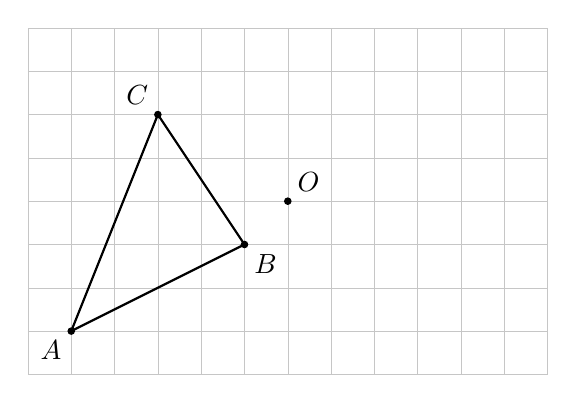
\begin{tikzpicture}[scale=0.55]
  \draw[gray!45,very thin] (0,0) grid (12,8);
  \draw[thick] (1,1)--(5,3)--(3,6)--cycle;
  \fill (6,4) circle (2.5pt) node[above right] {$O$};
  \fill (1,1) circle (2.5pt) node[below left] {$A$};
  \fill (5,3) circle (2.5pt) node[below right] {$B$};
  \fill (3,6) circle (2.5pt) node[above left] {$C$};
\end{tikzpicture}
\end{center}
\begin{enumerate}
  \item ابنِ النقاط $A'$ و $B'$ و $C'$ مناظرات $A$ و $B$ و $C$ على التوالي بالنسبة إلى $O$.
  \item قارن $A'B'$ و $AB$، ثم قارن اتجاهي $(AB)$ و $(A'B')$.
  \item $I$ منتصف $[AB]$. أين تقع مناظرة $I$ ؟ علّل.
\end{enumerate}
\axsol
\begin{enumerate}[itemsep=14pt]
  \item\leavevmode
  \begin{prop}[تعريف]
  \ib{$A'=S_O(A)$} معناه أن $O$ منتصف $[AA']$ : نمرّ من $A$ إلى $O$ ثم نواصل بنفس الانتقال.
  \end{prop}
  \begin{itemize}
    \item من $A$ إلى $O$ : 5 وحدات يمينا و 3 وحدات إلى الأعلى. نواصل من $O$ بنفس الانتقال فنجد $A'$.
    \item من $B$ إلى $O$ : وحدة يمينا ووحدة إلى الأعلى، وهكذا نجد $B'$.
    \item من $C$ إلى $O$ : 3 وحدات يمينا ووحدتان إلى الأسفل، وهكذا نجد $C'$.
  \end{itemize}
  \begin{center}
  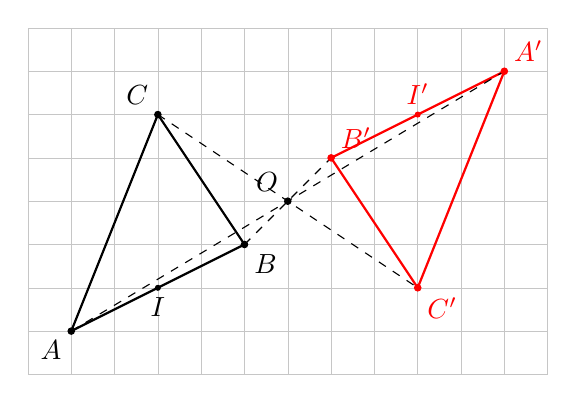
\begin{tikzpicture}[scale=0.55]
    \draw[gray!45,very thin] (0,0) grid (12,8);
    \draw[thick] (1,1)--(5,3)--(3,6)--cycle;
    \draw[thick,red] (11,7)--(7,5)--(9,2)--cycle;
    \draw[dashed] (1,1)--(11,7);
    \draw[dashed] (5,3)--(7,5);
    \draw[dashed] (3,6)--(9,2);
    \fill (6,4) circle (2.5pt) node[above left] {$O$};
    \fill (1,1) circle (2.5pt) node[below left] {$A$};
    \fill (5,3) circle (2.5pt) node[below right] {$B$};
    \fill (3,6) circle (2.5pt) node[above left] {$C$};
    \fill[red] (11,7) circle (2.5pt) node[above right] {$A'$};
    \fill[red] (7,5) circle (2.5pt) node[above right] {$B'$};
    \fill[red] (9,2) circle (2.5pt) node[below right] {$C'$};
    \fill (3,2) circle (2pt) node[below] {$I$};
    \fill[red] (9,6) circle (2pt) node[above] {$I'$};
  \end{tikzpicture}
  \end{center}
  \item \begin{prop}[الحفاظ على الأطوال]
  مناظر القطعة $[AB]$ هو القطعة $[A'B']$ ، و \ib{$A'B'=AB$} ، و $(A'B')\parallel(AB)$.
  \end{prop}
  على الشكل نلاحظ أن $A'B'=AB$ وأن $(A'B')$ يوازي $(AB)$ : الانتقال من $A'$ إلى $B'$ هو نفسه الانتقال من $B$ إلى $A$ (4 وحدات يسارا ووحدتان إلى الأسفل).
  \item التناظر المركزي يحافظ على منتصف القطعة. مناظر $I$ هي النقطة $I'$ التي تقع في منتصف $[A'B']$ : \ib{$I'$ منتصف $[A'B']$}.
\end{enumerate}
\end{corr}

\end{document}
